\documentclass[]{book}
\usepackage{lmodern}
\usepackage{amssymb,amsmath}
\usepackage{ifxetex,ifluatex}
\usepackage{fixltx2e} % provides \textsubscript
\ifnum 0\ifxetex 1\fi\ifluatex 1\fi=0 % if pdftex
  \usepackage[T1]{fontenc}
  \usepackage[utf8]{inputenc}
\else % if luatex or xelatex
  \ifxetex
    \usepackage{mathspec}
  \else
    \usepackage{fontspec}
  \fi
  \defaultfontfeatures{Ligatures=TeX,Scale=MatchLowercase}
\fi
% use upquote if available, for straight quotes in verbatim environments
\IfFileExists{upquote.sty}{\usepackage{upquote}}{}
% use microtype if available
\IfFileExists{microtype.sty}{%
\usepackage{microtype}
\UseMicrotypeSet[protrusion]{basicmath} % disable protrusion for tt fonts
}{}
\usepackage[margin=1in]{geometry}
\usepackage{hyperref}
\hypersetup{unicode=true,
            pdftitle={Internet of Things for Smart Industry},
            pdfauthor={Franz Maurer, Witek ten Hove \& Deny Smeets},
            pdfborder={0 0 0},
            breaklinks=true}
\urlstyle{same}  % don't use monospace font for urls
\usepackage{natbib}
\bibliographystyle{apalike}
\usepackage{longtable,booktabs}
\usepackage{graphicx,grffile}
\makeatletter
\def\maxwidth{\ifdim\Gin@nat@width>\linewidth\linewidth\else\Gin@nat@width\fi}
\def\maxheight{\ifdim\Gin@nat@height>\textheight\textheight\else\Gin@nat@height\fi}
\makeatother
% Scale images if necessary, so that they will not overflow the page
% margins by default, and it is still possible to overwrite the defaults
% using explicit options in \includegraphics[width, height, ...]{}
\setkeys{Gin}{width=\maxwidth,height=\maxheight,keepaspectratio}
\IfFileExists{parskip.sty}{%
\usepackage{parskip}
}{% else
\setlength{\parindent}{0pt}
\setlength{\parskip}{6pt plus 2pt minus 1pt}
}
\setlength{\emergencystretch}{3em}  % prevent overfull lines
\providecommand{\tightlist}{%
  \setlength{\itemsep}{0pt}\setlength{\parskip}{0pt}}
\setcounter{secnumdepth}{5}
% Redefines (sub)paragraphs to behave more like sections
\ifx\paragraph\undefined\else
\let\oldparagraph\paragraph
\renewcommand{\paragraph}[1]{\oldparagraph{#1}\mbox{}}
\fi
\ifx\subparagraph\undefined\else
\let\oldsubparagraph\subparagraph
\renewcommand{\subparagraph}[1]{\oldsubparagraph{#1}\mbox{}}
\fi

%%% Use protect on footnotes to avoid problems with footnotes in titles
\let\rmarkdownfootnote\footnote%
\def\footnote{\protect\rmarkdownfootnote}

%%% Change title format to be more compact
\usepackage{titling}

% Create subtitle command for use in maketitle
\newcommand{\subtitle}[1]{
  \posttitle{
    \begin{center}\large#1\end{center}
    }
}

\setlength{\droptitle}{-2em}
  \title{Internet of Things for Smart Industry}
  \pretitle{\vspace{\droptitle}\centering\huge}
  \posttitle{\par}
  \author{Franz Maurer, Witek ten Hove \& Deny Smeets}
  \preauthor{\centering\large\emph}
  \postauthor{\par}
  \predate{\centering\large\emph}
  \postdate{\par}
  \date{2017-06-06}

\usepackage{booktabs}
\usepackage{amsthm}
\makeatletter
\def\thm@space@setup{%
  \thm@preskip=8pt plus 2pt minus 4pt
  \thm@postskip=\thm@preskip
}
\makeatother

\usepackage{amsthm}
\newtheorem{theorem}{Theorem}[chapter]
\newtheorem{lemma}{Lemma}[chapter]
\theoremstyle{definition}
\newtheorem{definition}{Definition}[chapter]
\newtheorem{corollary}{Corollary}[chapter]
\newtheorem{proposition}{Proposition}[chapter]
\theoremstyle{definition}
\newtheorem{example}{Example}[chapter]
\theoremstyle{remark}
\newtheorem*{remark}{Remark}
\begin{document}
\maketitle

{
\setcounter{tocdepth}{1}
\tableofcontents
}
\chapter{Welcome}\label{welcome}

This is an accompanying book to the HAN Minor Smart Industry and covers
the major topics regarding the Internet of Things (IoT) implementation
in an industrial setting.

\chapter{Introduction to IoT}\label{intro}

The IoT is the product of physical objects, controllers, sensors and
actuators and the internet \citep{mcewen_designing_2013}. The first
reference to the IoT was in 1982, when researchers at Carnegie Mellon
University developed the world's first IoT-enabled Coke Machine. Mark
Weiser developed the concept further in the early 90s; and Kevin Ashton
coined the term `Internet of Things' around 1999.

\chapter{IoT Capabilities}\label{capabilities}

 Your browser does not support this format.

\chapter{IoT Framework}\label{framework}

We describe our methods in this chapter.

\chapter{IoT Markets}\label{markets}

Some \emph{significant} applications are demonstrated in this chapter.

\section{Example one}\label{example-one}

\section{Example two}\label{example-two}

\chapter{IoT Fundamentals}\label{fundamentals}

We have finished a nice book.

\chapter{Sensors}\label{sensors}

We have finished a nice book.

\hypertarget{communication}{\chapter{Data
Communication}\label{communication}}

We have finished a nice book.

\chapter{Cloud Storage}\label{cloud}

After sensors start to send data it is necessary that you define a place
where that data should be stored. In the context of IoT the Cloud is a
place somewhere on the internet where a provider allows recognized
sensors to store their raw data in a database. You as the owner has
access to that database, are able to program it and know how results
could be made visible on dashboards. So it is not necessary anymore to
maintain your own private servers in your own data centers, but cloud
platform companies are now taking over that role.

Raw data is in fact meaningless. You will have to analyze it, reshuffle,
run statistics on it, correlate it with other data, watch for
exceptional values and so on to make raw sensor data valuable for your
business goals. We will touch on data analytics, machine learning and
data science in \protect\hyperlink{analytics}{section 13}.

In this chapter we will look into data, their place in the IoT
infrastructure and explore one of the many cloud solutions.

\section{Database Systems}\label{database-systems}

As most IoT devices have very limited memory resources, the data they
produce has to be stored elsewhere. We discussed the data communication
possibilities in \protect\hyperlink{communication}{section 8}. In theory
the data could be gathered into a simple text file and applications
could read from this source.

However we soon would encounter some annoying practical problems. For
instance while data is written to a text file it is blocked. This would
mean other devices can not add their data resulting in data loss. Also a
text file is not the most efficient user of memory and its size would
grow exponentially when used in a professional application with large
numbers of devices and users. Other issues include lack of search and
filtering facilities and connecting to other data tables.

The above mentioned problems are not uniquely related to the IoT system.
It translates to any client server environment. Database systems have
been developed to cope with the challenges of efficiently creating large
quantities of data, read records, and update and delete them. These
basic database functionalities have been summarized in the CRUD acronym.

The most common language for doing CRUD operations on a database is SQL
(Structured Query Language). It has a rather human friendly syntax. For
example this is the instruction for retrieving a selection of data from
a data table (What do you think it will return?):

\begin{verbatim}
SELECT * FROM SensorData WHERE Weekday = 'Monday'
\end{verbatim}

\begin{table}

\caption{\label{tab:dbtable}An example database table: SensorData}
\centering
\begin{tabular}[t]{llr}
\toprule
DeviceID & Weekday & Temperature\\
\midrule
B4 & Monday & -8.5\\
A1 & Monday & -8.0\\
B4 & Monday & -8.5\\
B1 & Monday & -8.2\\
B1 & Monday & -8.8\\
\addlinespace
A3 & Monday & -8.8\\
B1 & Monday & -8.6\\
B3 & Monday & -8.6\\
B2 & Tuesday & -8.3\\
A3 & Tuesday & -9.0\\
B2 & Tuesday & -8.8\\
\bottomrule
\end{tabular}
\end{table}

A database consists of many tables. These tables can be related through
key variables. For instance one table can contain sensor data while
another table contains the meta data per device. These tables can be
combined via a shared variable (\emph{field}) containing the device IDs.
When the meta data includes location data (e.g.~longitude/latitude) you
could draw maps with the temperature measurements.

Databases that follow the above described structure belong to the
category of Relational Database Systems (RDBS). Popular (open source)
instances are \href{https://www.postgresql.org/}{PostgreSQL} and
\href{https://www.mysql.com/}{MySQL}. Another category of database
systems that is gaining attention are the NoSQL systems. An example is
\href{https://www.mongodb.com/}{MongoDB} (also open source). An
important difference between the two categories is that an RDBS can only
hold one value per cell in a table (like a spreadsheet), whereas a NoSQL
database can hold nested vectors of values in one cell (like
\href{http://www.json.org/}{JSON}).

\begin{verbatim}
## [
##   {
##     "DeviceID": "A1",
##     "Weekday": "Monday",
##     "Temperature": [-8]
##   },
##   {
##     "DeviceID": "A3",
##     "Weekday": "Monday",
##     "Temperature": [-8.8]
##   },
##   {
##     "DeviceID": "B1",
##     "Weekday": "Monday",
##     "Temperature": [-8.2, -8.8, -8.6]
##   },
##   {
##     "DeviceID": "B3",
##     "Weekday": "Monday",
##     "Temperature": [-8.6]
##   },
##   {
##     "DeviceID": "B4",
##     "Weekday": "Monday",
##     "Temperature": [-8.5, -8.5]
##   }
## ]
\end{verbatim}

\citep[Video:][]{google_developers_google_nodate}

Another interesting alternative database architecture is the graph
database. In a graph database data is represented as a network where the
records are stored in nodes and the relationships in the edges. This is
a very convenient solution when you are more interested in the
relationships between objects rather than doing aggregations on the
objects (sums, averages, etc).

\citep[Video:][]{neo4j_-_the_worlds_leading_graph_database_intro_nodate}

\section{Things in a network}\label{things-in-a-network}

\section{Amazon Web Services}\label{amazon-web-services}

\chapter{Privacy}\label{privacy}

We have finished a nice book.

\chapter{Security}\label{security}

We have finished a nice book.

\chapter{Encryption}\label{encryption}

We have finished a nice book.

\hypertarget{analytics}{\chapter{Data Analytics}\label{analytics}}

\begin{figure}[htbp]
\centering
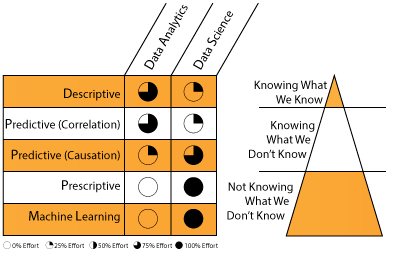
\includegraphics{./images/datascience.png}
\caption{Fig.12.1 - Data Analytics versus Science}
\end{figure}

\citep{j_data_2013}

\chapter{Dashboards and Apps}\label{apps}

We have finished a nice book.

\chapter{Open Source Systems}\label{opensource}

We have finished a nice book.

\chapter{Arduino Programming}\label{arduino}

We have finished a nice book.

\bibliography{packages.bib,book.bib}


\end{document}
